\chapter{Leçon 32: Virbereedung op de Sproochentest: Meng Aarbecht a Bildbeschreiwung}

Dës Lektioun ass eng geziilt Virbereedung op de mündleche Sproochentest fir d'Lëtzebuerger Nationalitéit. Mir behandelen zwee zentral Deeler vun der Prüfung: den éischten Deel mat Froen an Äntwerten iwwer d'Thema \textbf{Meng Aarbecht}, an den zweeten Deel mat enger detailléierter Bildbeschreiwung vun enger Familljekichen. Zousätzlech bespriechen mir d'Sproochtipps, d'Eifeler Regel, d'Benotzung vum Präsens mat \textbf{säit}, den Ënnerscheed tëscht \textbf{e Rank} (bague/ring) an \textbf{e Rack} (robe/dress), sou wéi wichteg Vokabelen an Ausdréck.

\textit{Cette leçon constitue une préparation ciblée à l'épreuve orale du Sproochentest pour l'obtention de la nationalité luxembourgeoise. Nous traitons deux parties centrales de l'examen : la première partie avec des questions et réponses sur le thème \textbf{Mon travail}, et la deuxième partie consacrée à la description détaillée d'une image représentant une cuisine familiale. Nous abordons également des points de grammaire importants, la règle d'Eifel, l'utilisation du présent avec \textbf{säit}, la différence entre \textbf{e Rank} (une bague/un anneau) et \textbf{e Rack} (une robe), ainsi que le vocabulaire clé.}

\textit{This lesson is a targeted preparation for the oral Sproochentest exam for Luxembourgish citizenship. We cover two core components of the exam: Part 1 featuring questions and answers on the topic \textbf{My Work}, and Part 2 featuring a detailed description of a family kitchen scene. Additionally, we discuss key grammar tips, the Eifeler rule, using the present tense with \textbf{säit}, the distinction between \textbf{e Rank} (a ring) and \textbf{e Rack} (a dress), as well as essential vocabulary.}

\vspace{1.5em}

\section[Sproochentest Deel 1: Meng Aarbecht / Q\&A]{Sproochentest Deel 1: Meng Aarbecht \\/ Questions et réponses : Mon travail \\/ Questions and Answers: My Work}

\noindent\textbf{1. Wat sidd Dir vu Beruff? / Als wat schafft Dir elo?}\\
\textit{(FR: Quelle est votre profession ? / Que faites-vous comme travail actuellement ? — EN: What is your profession? / What do you do for work currently?)}\\[0.3em]
\textit{Ech si Projektmanagerin bei enger Bank zu Lëtzebuerg.}\\
\textit{Ech} (Je / I) \textit{si} (suis / am) \textit{Projektmanagerin} (gestionnaire de projet / project manager) \textit{bei enger Bank} (dans une banque / at a bank) \textit{zu Lëtzebuerg} (au Luxembourg / in Luxembourg).\\
$\rightarrow$ Français : \textit{Je suis chef de projet dans une banque au Luxembourg.}\\
$\rightarrow$ English : \textit{I am a project manager at a bank in Luxembourg.}\\[0.8em]

\noindent\textbf{2. Wou schafft Dir am Moment? Wou ass Äre Büro?}\\
\textit{(FR: Où travaillez-vous en ce moment ? Où se trouve votre bureau ? — EN: Where do you work at the moment? Where is your office?)}\\[0.3em]
\textit{Ech schaffe bei der Deutsche Börse um Kirchberg zu Lëtzebuerg.}\\
\textit{Ech schaffe} (Je travaille / I work) \textit{bei der Deutsche Börse} (chez Deutsche Börse / at Deutsche Börse) \textit{um Kirchberg} (au Kirchberg / in Kirchberg) \textit{zu Lëtzebuerg} (à Luxembourg / in Luxembourg).\\
$\rightarrow$ Français : \textit{Je travaille chez Deutsche Börse au Kirchberg à Luxembourg.}\\
$\rightarrow$ English : \textit{I work at Deutsche Börse in Kirchberg, Luxembourg.}\\[0.8em]

\noindent\textbf{3. Säit wéini schafft Dir do? / Wéi laang schafft Dir schonn do?}\\
\textit{(FR: Depuis quand travaillez-vous là-bas ? / Depuis combien de temps y travaillez-vous ? — EN: Since when have you been working there? / How long have you been working there?)}\\[0.3em]
\textit{Ech schaffe säit 2021 do. / Ech schaffe säit fënnef Joer do.}\\
\textit{Ech schaffe} (Je travaille [présent!] / I work [present tense!]) \textit{säit 2021} (depuis 2021 / since 2021) \textit{do} (là / there).\\
$\rightarrow$ Français : \textit{Je travaille là-bas depuis 2021. (Attention : en luxembourgeois, on utilise le présent avec « säit » quand l'action continue !)}\\
$\rightarrow$ English : \textit{I have been working there since 2021. (Note: Luxembourgish uses the present tense with "säit" for ongoing actions!)}\\[0.8em]

\noindent\textbf{4. Wéi gitt / fuert Dir op d'Aarbecht?}\\
\textit{(FR: Comment allez-vous au travail ? — EN: How do you get to work?)}\\[0.3em]
\textit{Normalerweis fueren ech mam Bus / huelen ech de Bus.}\\
\textit{Normalerweis} (Normalement / Normally) \textit{fueren ech mam Bus} (je vais en bus / I go by bus) \textit{/ huelen ech de Bus} (ou je prends le bus / or I take the bus).\\
$\rightarrow$ Français : \textit{Normalement, je vais au travail en bus / je prends le bus.}\\
$\rightarrow$ English : \textit{Normally, I travel to work by bus / I take the bus.}\\[0.8em]

\noindent\textbf{5. Wéi laang braucht Dir fir op d'Aarbecht ze kommen?}\\
\textit{(FR: Combien de temps vous faut-il pour arriver au travail ? — EN: How long does it take you to get to work?)}\\[0.3em]
\textit{Ech brauche meeschtens ongeféier drësseg Minutten (eng hallef Stonn) fir op d'Aarbecht ze kommen.}\\
\textit{Ech brauche} (J'ai besoin de, il me faut / I need, it takes me) \textit{meeschtens} (la plupart du temps / mostly) \textit{ongeféier} (environ / approximately) \textit{drësseg Minutten} (trente minutes / thirty minutes) \textit{(eng hallef Stonn)} (une demi-heure / half an hour) \textit{fir op d'Aarbecht ze kommen} (pour arriver au travail / to get to work).\\
$\rightarrow$ Français : \textit{Il me faut généralement environ trente minutes (une demi-heure) pour arriver au travail.}\\
$\rightarrow$ English : \textit{It usually takes me about thirty minutes (half an hour) to get to work.}\\[0.8em]

\noindent\textbf{6. Um wéi vill Auer fänkt Dir un ze schaffen? Um wéi vill Auer maacht Dir Feierowend?}\\
\textit{(FR: À quelle heure commencez-vous à travailler ? À quelle heure finissez-vous votre journée ? — EN: What time do you start work? What time do you finish work?)}\\[0.3em]
\textit{Ech fänken um 8 Auer moies un an ech maache um 5 Auer (17.00 Auer) am Nomëtteg Feierowend.}\\
\textit{Ech fänken... un} (Je commence / I start) \textit{um 8 Auer moies} (à 8 heures du matin / at 8 a.m.) \textit{an ech maache Feierowend} (et je finis ma journée de travail / and I finish work) \textit{um 5 Auer am Nomëtteg} (à 17 heures / at 5 p.m.).\\
$\rightarrow$ Français : \textit{Je commence à 8 heures du matin et je finis le travail à 17 heures.}\\
$\rightarrow$ English : \textit{I start at 8 a.m. and I finish work at 5 p.m.}\\[0.8em]

\noindent\textbf{7. Wat sinn Är typesch Aktivitéiten op der Aarbecht?}\\
\textit{(FR: Quelles sont vos activités typiques au travail ? — EN: What are your typical activities at work?)}\\[0.3em]
\textit{Ech plangen Aktivitéiten a Reunioune mat menge Kollegen. Ech schreiwe Berichter an ech kommunizéiere mat verschiddenen Ekippen.}\\
\textit{Ech plangen} (Je planifie / I plan) \textit{Aktivitéiten a Reuniounen} (des activités et des réunions / activities and meetings) \textit{mat menge Kollegen} (avec mes collègues / with my colleagues). \textit{Ech schreiwen} (J'écris / I write) \textit{Berichter} (des rapports / reports) \textit{an ech kommunizéieren} (et je communique / and I communicate) \textit{mat verschiddenen Ekippen} (avec différentes équipes / with various teams).\\
$\rightarrow$ Français : \textit{Je planifie des activités et des réunions avec mes collègues. J'écris des rapports et je communique avec différentes équipes.}\\
$\rightarrow$ English : \textit{I plan activities and meetings with my colleagues. I write reports and communicate with different teams.}\\[0.8em]

\noindent\textbf{8. Wat gefält Iech an Ärer Aarbecht a wat net?}\\
\textit{(FR: Qu'aimez-vous dans votre travail et qu'aimez-vous moins ? — EN: What do you like about your job and what do you not like?)}\\[0.3em]
\textit{Mir gefält d'Ambiance, well ech gär mat menge Kollegen discutéieren an an enger Ekipp schaffen. Wat mir manner gefält ass, datt et heiansdo ze vill Drock a Stress gëtt.}\\
\textit{Mir gefält} (J'aime, cela me plaît / I like) \textit{d'Ambiance} (l'ambiance / the atmosphere), \textit{well ech gär} (parce que j'aime bien / because I like to) \textit{mat menge Kollegen discutéieren} (discuter avec mes collègues / chat with my colleagues) \textit{an an enger Ekipp schaffen} (et travailler en équipe / and work in a team). \textit{Wat mir manner gefält} (Ce qui me plaît moins / What I like less) \textit{ass, datt et heiansdo} (est qu'il y a parfois / is that sometimes there is) \textit{ze vill Drock a Stress gëtt} (trop de pression et de stress / too much pressure and stress).\\
$\rightarrow$ Français : \textit{J'aime l'ambiance parce que j'apprécie discuter avec mes collègues et travailler en équipe. Ce qui me plaît moins, c'est qu'il y a parfois trop de pression et de stress.}\\
$\rightarrow$ English : \textit{I like the atmosphere because I enjoy chatting with my colleagues and working in a team. What I like less is that sometimes there is too much pressure and stress.}\\[0.8em]

\noindent\textbf{9. Wat mécht Är Firma?}\\
\textit{(FR: Que fait votre entreprise ? — EN: What does your company do?)}\\[0.3em]
\textit{Eis Firma ass en Intermédiaire um Finanzmaart a gehéiert zum Grupp vun der Deutsche Börse.}\\
\textit{Eis Firma} (Notre entreprise / Our company) \textit{ass en Intermédiaire} (est un intermédiaire / is an intermediary) \textit{um Finanzmaart} (sur le marché financier / in the financial market) \textit{a gehéiert} (et appartient / and belongs) \textit{zum Grupp vun der Deutsche Börse} (au groupe Deutsche Börse / to the Deutsche Börse Group).\\
$\rightarrow$ Français : \textit{Notre entreprise est un intermédiaire sur le marché financier et fait partie du groupe Deutsche Börse.}\\
$\rightarrow$ English : \textit{Our company is an intermediary in the financial market and is part of the Deutsche Börse Group.}\\[0.8em]

\noindent\textbf{10. Um wéi vill Auer hutt Dir Mëttespaus a wéi laang dauert se?}\\
\textit{(FR: À quelle heure avez-vous votre pause déjeuner et combien de temps dure-t-elle ? — EN: What time do you have your lunch break and how long does it last?)}\\[0.3em]
\textit{Ech hu meng Mëttespaus vun 12.00 bis 13.00 Auer. Se dauert eng Stonn.}\\
\textit{Ech hu} (J'ai / I have) \textit{meng Mëttespaus} (ma pause déjeuner / my lunch break) \textit{vun 12.00 bis 13.00 Auer} (de 12h à 13h / from 12 to 1 p.m.). \textit{Se dauert} (Elle dure / It lasts) \textit{eng Stonn} (une heure / one hour).\\
$\rightarrow$ Français : \textit{J'ai ma pause déjeuner de 12h à 13h. Elle dure une heure.}\\
$\rightarrow$ English : \textit{I have my lunch break from 12 to 1 p.m. It lasts one hour.}\\[0.8em]

\noindent\textbf{11. Hutt Dir eng Kantin op der Aarbecht?}\\
\textit{(FR: Avez-vous une cantine au travail ? — EN: Do you have a canteen at work?)}\\[0.3em]
\textit{Jo, mir hunn eng grouss a ganz gutt Kantin mat vill Auswiel.}\\
\textit{Jo} (Oui / Yes), \textit{mir hunn} (nous avons / we have) \textit{eng grouss a ganz gutt Kantin} (une grande et très bonne cantine / a large and very good canteen) \textit{mat vill Auswiel} (avec beaucoup de choix / with plenty of choices).\\
$\rightarrow$ Français : \textit{Oui, nous avons une grande et très bonne cantine avec beaucoup de choix.}\\
$\rightarrow$ English : \textit{Yes, we have a large and very good canteen with plenty of choices.}\\[0.8em]

\noindent\textbf{12. Musst Dir heiansdo Iwwerstonne schaffen?}\\
\textit{(FR: Devez-vous parfois faire des heures supplémentaires ? — EN: Do you sometimes have to work overtime?)}\\[0.3em]
\textit{Dat hänkt dovun of: wann et vill Aarbecht um Projet gëtt, muss ech heiansdo Iwwerstonne maachen.}\\
\textit{Dat hänkt dovun of} (Cela dépend / That depends): \textit{wann et vill Aarbecht... gëtt} (quand il y a beaucoup de travail / when there is a lot of work), \textit{muss ech} (je dois / I must) \textit{Iwwerstonne maachen} (faire des heures supplémentaires / work overtime).\\
$\rightarrow$ Français : \textit{Cela dépend : s'il y a beaucoup de travail sur le projet, je dois parfois faire des heures supplémentaires.}\\
$\rightarrow$ English : \textit{That depends: if there is a lot of work on the project, I sometimes have to work overtime.}\\[0.8em]

\noindent\textbf{13. Hutt Dir en Dresscode op der Aarbecht?}\\
\textit{(FR: Avez-vous un code vestimentaire au travail ? — EN: Do you have a dress code at work?)}\\[0.3em]
\textit{Mir hu kee ganz strikten Dresscode, mä mir kleeden eis propper an « business casual ».}\\
\textit{Mir hu kee} (Nous n'avons pas de / We do not have a) \textit{strikten Dresscode} (code vestimentaire strict / strict dress code), \textit{mä mir kleeden eis} (mais nous nous habillons / but we dress) \textit{propper} (proprement, correctement / neatly, properly) \textit{a « business casual »}.\\
$\rightarrow$ Français : \textit{Nous n'avons pas de code vestimentaire très strict, mais nous nous habillons de manière propre et « business casual ».}\\
$\rightarrow$ English : \textit{We don't have a very strict dress code, but we dress neatly and "business casual".}

\vspace{1.5em}

\section[Sproochentest Deel 2: Bildbeschreiwung (Familljekichen) / Picture Description]{Sproochentest Deel 2: Bildbeschreiwung (Familljekichen) \\/ Description d'image : Cuisine familiale \\/ Picture Description: Family Kitchen}

\begin{center}
\includegraphics[width=0.75\textwidth]{tasks/img\_famill.png} \\
\textit{Bild: Eng Famill mat zwee Kanner an der Kichen / Image : Une famille avec deux enfants dans la cuisine / Picture: A family with two children in the kitchen}
\end{center}

\vspace{1em}

\subsection*{Mëndlech Beschreiwung fir de Sproochentest (Modelltext / Text Model)}

\noindent\textbf{1. Allgemeine Androck (Vue d'ensemble / Overview):}\\
Um Bild gesäit een eng Famill vu véier Leit (e Papp, eng Mamm an zwee kleng Kanner) doheem an enger moderner Kichen am Summer. Déi ganz Famill ass frou a laacht.\\
$\rightarrow$ Français : \textit{Sur l'image, on voit une famille de quatre personnes (un père, une mère et deux jeunes enfants) à la maison dans une cuisine moderne en été. Toute la famille est joyeuse et sourit.}\\
$\rightarrow$ English : \textit{In the picture, one sees a family of four people (a father, a mother, and two young children) at home in a modern kitchen in summer. The whole family is happy and smiling.}\\[0.5em]

\noindent\textbf{2. Beschreiwung vun de Persounen (Description des personnes / Description of people):}
\begin{itemize}
    \item \textbf{De Papp (Le père / The father):} Hien ass ongeféier 40 Joer al an huet eng Glatz an e schwaarze Baart. Hien dréit e wäisst Hiem an eng blo-wäiss kariéiert Box mat groë Strëmp. Hien hält säi klenge Jong op der Hëft (am Aarm) an hie kritt e Stéck Brout vu senger Fra gefiddert.\\
    $\rightarrow$ Français : \textit{Il a environ 40 ans, est chauve et porte une barbe noire. Il porte une chemise blanche et un short quadrillé bleu et blanc avec des chaussettes grises. Il tient son petit garçon sur la hanche et sa femme lui donne un morceau de pain.}\\
    $\rightarrow$ English : \textit{He is about 40 years old, bald, and has a black beard. He wears a white shirt and blue-and-white checked shorts with gray socks. He holds his little boy on his hip and his wife feeds him a piece of bread.}
    
    \item \textbf{D'Mamm (La mère / The mother):} Si ass ongeféier 30–35 Joer al a ganz elegant. Si dréit e gesträift blo-wäisst Kleed. Si ass schwanger (si erwaart e Puppelchen!). Si fiddert hirem Mann e Stéck Brout mat Schockelascreme (Nutella) a laacht.\\
    $\rightarrow$ Français : \textit{Elle a environ 30-35 ans et est très élégante. Elle porte une robe rayée bleue et blanche. Elle est enceinte (elle attend un bébé !). Elle donne un morceau de pain avec de la pâte à tartiner au chocolat à son mari et sourit.}\\
    $\rightarrow$ English : \textit{She is about 30–35 years old and very elegant. She wears a striped blue-and-white dress. She is pregnant (expecting a baby!). She feeds her husband a piece of bread with chocolate spread (Nutella) and smiles.}
    
    \item \textbf{D'Duechter (La fille / The daughter):} Lénks steet e klengt Meedche vu fënnef Joer al mat laangen donkelen Hoer an enger wäisser Spang (\textit{eng Spang / e Spängelchen}). Si dréit e rosa Kleedchen an e Schiertech (\textit{e Schiertech}). Si schmiert mat engem Messer Schockelascreme op e Stéck Brout op engem Schneidbriet (\textit{e Schneidbriet}).\\
    $\rightarrow$ Français : \textit{À gauche se trouve une petite fille de 5 ans avec de longs cheveux foncés et une barrette blanche. Elle porte une petite robe rose et un tablier. Elle étale de la pâte au chocolat avec un couteau sur un morceau de pain sur une planche à découper.}\\
    $\rightarrow$ English : \textit{On the left stands a 5-year-old little girl with long dark hair and a white hair clip. She wears a little pink dress and an apron. She spreads chocolate cream with a knife on a piece of bread on a cutting board.}
    
    \item \textbf{De klenge Jong / Puppelchen (Le petit garçon / The baby boy):} Riets ass e klenge Jong vun engem Joer al mat gekrauselten Hoer. Hien dréit e wäisst Hiemchen an ass um Aarm vu sengem Papp.\\
    $\rightarrow$ Français : \textit{À droite se trouve un petit garçon d'un an aux cheveux bouclés. Il porte une petite chemise blanche et est dans les bras de son père.}\\
    $\rightarrow$ English : \textit{On the right is a one-year-old little boy with curly hair. He wears a little white shirt and is held in his father's arms.}
\end{itemize}

\noindent\textbf{3. Kichenraum an Detailer (Environnement et détails / Environment and details):}
\begin{itemize}
    \item Si stinn bei enger Kicheninsel/Aarbechtsplack. Op der Aarbechtsplack steet e Glaskragel Schockela (Nutella), eng geschnidde Baguette, e Messer, e Salzstreeër an eng wäiss Tass.\\
    $\rightarrow$ Français : \textit{Ils se tiennent près d'un îlot de cuisine / plan de travail. Sur le plan de travail se trouvent un pot de Nutella, une baguette coupée, un couteau, une salière et une tasse blanche.}\\
    $\rightarrow$ English : \textit{They stand near a kitchen island / countertop. On the countertop is a jar of Nutella, a sliced baguette, a knife, a salt shaker, and a white mug.}

    \item Am Hannergrond gesäit een eng rout Ziegelmauer, grouss Fënsteren, an zwou rout Luuchten déi ugesteckt sinn. Dohanner sinn e Kachuewen an eng Orchidee op engem Regal.\\
    $\rightarrow$ Français : \textit{En arrière-plan, on voit un mur de briques rouges, de grandes fenêtres et deux lampes rouges allumées. Derrière se trouvent une cuisinière et une orchidée sur une étagère.}\\
    $\rightarrow$ English : \textit{In the background, one sees a red brick wall, large windows, and two lit red lamps. Behind them are a stove and an orchid on a shelf.}
\end{itemize}

\noindent\textbf{4. Wichteg Ausdréck fir den Examen (Phrases clés pour l'examen / Key exam phrases):}
\begin{itemize}
    \item \textit{Um Bild gesäit een...} (Sur l'image, on voit... / In the picture, one sees...)
    \item \textit{Am Virgrond / Am Hannergrond...} (Au premier plan / Au second plan... / In the foreground / background...)
    \item \textit{Op der lénker Säit / Op der rietser Säit...} (Sur le côté gauche / droit... / On the left / right side...)
    \item \textit{Ech mengen, datt si eppes z'iesse maachen.} (Je pense qu'ils préparent quelque chose à manger. / I think they are preparing something to eat.)
\end{itemize}

\vspace{1.5em}

\section[Grammaire a Sproochtipps / Grammar \& Tips]{Grammaire a Sproochtipps \\/ Points de grammaire et conseils \\/ Grammar Points and Language Tips}

\subsection*{1. Den Ënnerscheed tëscht « e Rank » an « e Rack » (Distinction entre « e Rank » et « e Rack » / Distinction between "e Rank" and "e Rack")}

\noindent\textit{Français : En luxembourgeois, il faut bien distinguer le sens des deux mots :}\\
\textit{English: In Luxembourgish, pay attention to the difference between these two words:}
\begin{itemize}
    \item \textbf{E Rank} (masculin, Plural: \textit{d'Räng} / \textit{d'Rénge}) = Un anneau, une bague / A ring, a hoop.
    \item \textbf{E Rack} (masculin, Plural: \textit{d'Räck}) = Une robe / A dress, a gown.
\end{itemize}
\textit{Beispill / Exemple / Example:}\\
\textit{D'Mamm dréit e schéine \textbf{Rack} an um Fanger dréit si e gëllene \textbf{Rank}.}\\
$\rightarrow$ Français : \textit{La mère porte une belle robe et au doigt elle porte une bague en or.}\\
$\rightarrow$ English : \textit{The mother wears a beautiful dress and on her finger she wears a gold ring.}

\subsection*{2. Benotzung vum Präsens mat « säit » (Utilisation du présent avec « säit » / Use of Present Tense with "säit")}

\noindent\textit{Français : En luxembourgeois, on utilise le \textbf{présent} avec « säit » lorsqu'une action commencée dans le passé se poursuit toujours dans le présent. En revanche, si l'action est terminée et ne continue plus aujourd'hui, on utilise le \textbf{passé composé} (sans « säit »).}\\
\textit{English: In Luxembourgish, the \textbf{present tense} is used with "säit" when an action started in the past is still ongoing in the present. If the action is finished and no longer continues today, use the \textbf{passé composé} (without "säit").}

\begin{itemize}
    \item \textbf{Präsens + säit (Lafend Handlung / Action toujours en cours / Still ongoing action):}\\
    \textit{Ech schaffe säit 2021 do.}\\
    $\rightarrow$ Français : \textit{Je travaille là-bas depuis 2021 (J'y ai commencé en 2021 et j'y travaille TOUJOURS aujourd'hui !)}\\
    $\rightarrow$ English : \textit{I have been working there since 2021 (I started in 2021 and I STILL work there today!)}
    
    \item \textbf{Passé composé (Ofgeschloss Handlung / Action terminée / Completed action):}\\
    \textit{Ech hunn do geschafft.}\\
    $\rightarrow$ Français : \textit{J'ai travaillé là-bas (C'est terminé dans le passé, je n'y travaille PLUS aujourd'hui !)}\\
    $\rightarrow$ English : \textit{I worked there (It is completed in the past, I do NOT work there anymore!)}
\end{itemize}

\subsection*{3. Eifeler Regel (n-Rule): « fueren ech » vs « ech fuere »}

\noindent\textit{Français : En luxembourgeois, le \textbf{-n} final est conservé devant les voyelles (a, e, i, o, u, y), les consonnes d, t, z, h, et la ponctuation. Devant les autres consonnes, le -n tombe.}\\
\textit{English: In Luxembourgish, the final \textbf{-n} is kept before vowels (a, e, i, o, u, y), the consonants d, t, z, h, and punctuation. Before other consonants, the final -n is dropped.}

\begin{itemize}
    \item \textbf{Richteg:} Normalerweis \textbf{fueren} ech... (\textit{Français : conserve le -n devant voyelle « e » / English: keeps -n before vowel "e"})
    \item \textbf{Richteg:} Ech \textbf{fuere} mam Bus... (\textit{Français : perd le -n devant consonne « m » / English: drops -n before consonant "m"})
    \item \textbf{Richteg:} Ech \textbf{huelen} de Bus... (\textit{Français : conserve le -n devant consonne « d » / English: keeps -n before consonant "d"})
    \item \textbf{Richteg:} Ech maache \textbf{Feierowend}... (\textit{Français : perd le -n devant consonne « f » / English: drops -n before consonant "f"})
    \item \textbf{Richteg:} vu \textbf{sengem} Papp... (\textit{Français : perd le -n devant consonne « s » / English: drops -n before consonant "s"})
\end{itemize}

\subsection*{4. Diminutiver an d'Grammatik: Neutrum « Meedche / Meedchen »}

\noindent\textit{Français : Les diminutifs en « -chen / -che » gardent généralement le genre de leur nom de base, mais \textbf{e Meedchen / e Meedche} (une fille) est neutre. Selon la règle d'Eifel, le -n final tombe devant une consonne.}\\
\textit{English: Diminutives ending in "-chen / -che" usually retain their base noun gender, but \textbf{e Meedchen / e Meedche} (a girl) is neuter. According to the n-Rule, the final -n drops before a consonant.}

\begin{itemize}
    \item \textbf{Richteg:} Lénks steet \textbf{e klengt Meedche} vu fënnef Joer. (\textit{Français : adjectif neutre « klengt », perd le -n devant consonne « v » / English: neuter adjective "klengt", drops -n before consonant "v"})
    \item \textbf{Richteg:} Hien dréit e wäisst \textbf{Hiemchen} an ass vu sengem Papp gehal... (\textit{Français : adjectif neutre « wäisst », conserve le -n devant voyelle « a » / English: neuter adjective "wäisst", keeps -n before vowel "a"})
\end{itemize}

\vspace{1.5em}

\section[Vokabelen / Vocabulaire / Vocabulary]{Vokabelen \\/ Vocabulaire illustré \\/ Illustrated Vocabulary}

Hei ass d'illustréiert Vokabellëscht vun de meescht benotzte Wierder aus eiser Virbereedungssessioun. \\
\textit{Voici la liste de vocabulaire illustré pour les mots clés étudiés. / Here is the illustrated vocabulary list for the key items discussed.}

\vspace{1.5em}

\begin{center}
    \begin{minipage}[t]{0.48\textwidth}
        \centering
        \textbf{Eng Spang}
        \vspace{0.5em}
        \framebox{\parbox{0.9\linewidth}{\centering
            \vspace{0.3cm}
            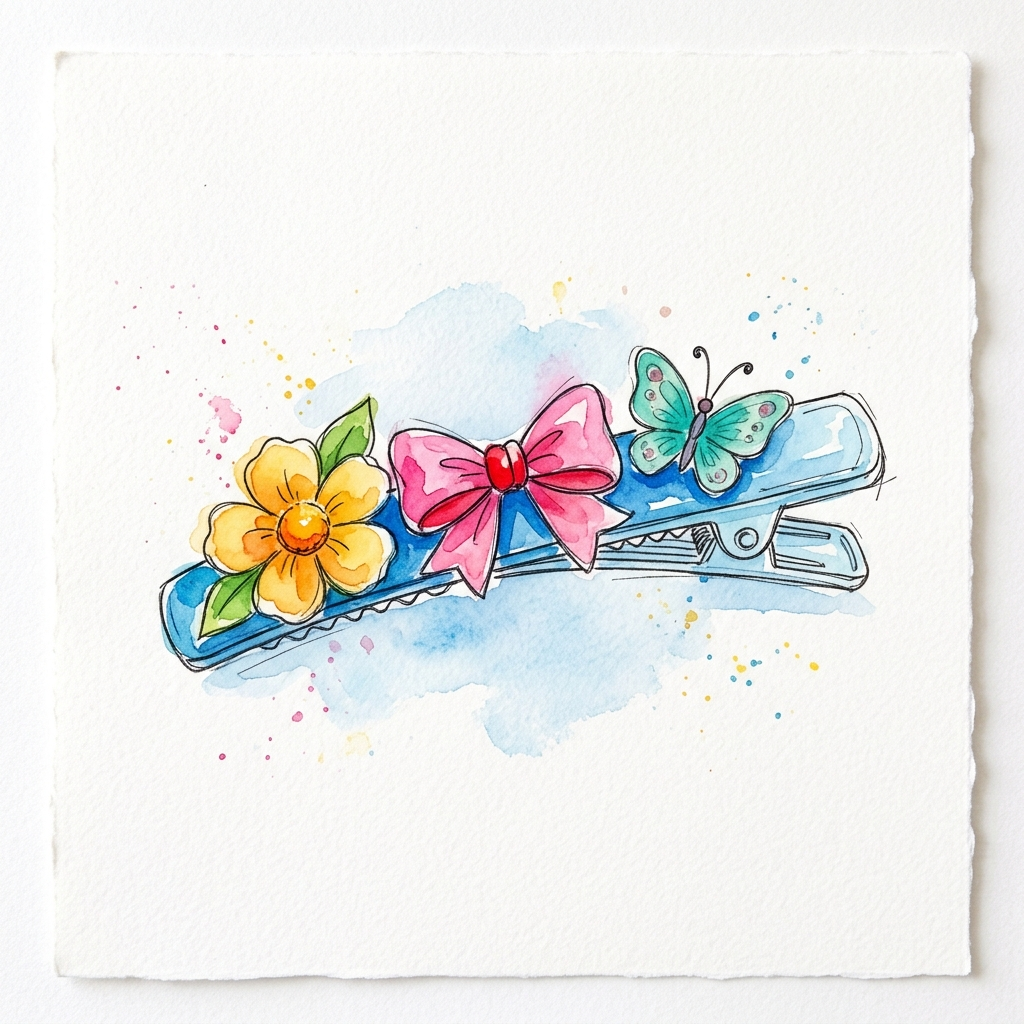
\includegraphics[width=0.85\linewidth,height=4cm,keepaspectratio]{vokab_300dpi/spang.png} \\
            \small\textit{D'Spang (Barrette / Hair clip)}
            \vspace{0.3cm}
        }}
    \end{minipage}
    \hfill
    \begin{minipage}[t]{0.48\textwidth}
        \centering
        \textbf{E Schiertech}
        \vspace{0.5em}
        \framebox{\parbox{0.9\linewidth}{\centering
            \vspace{0.3cm}
            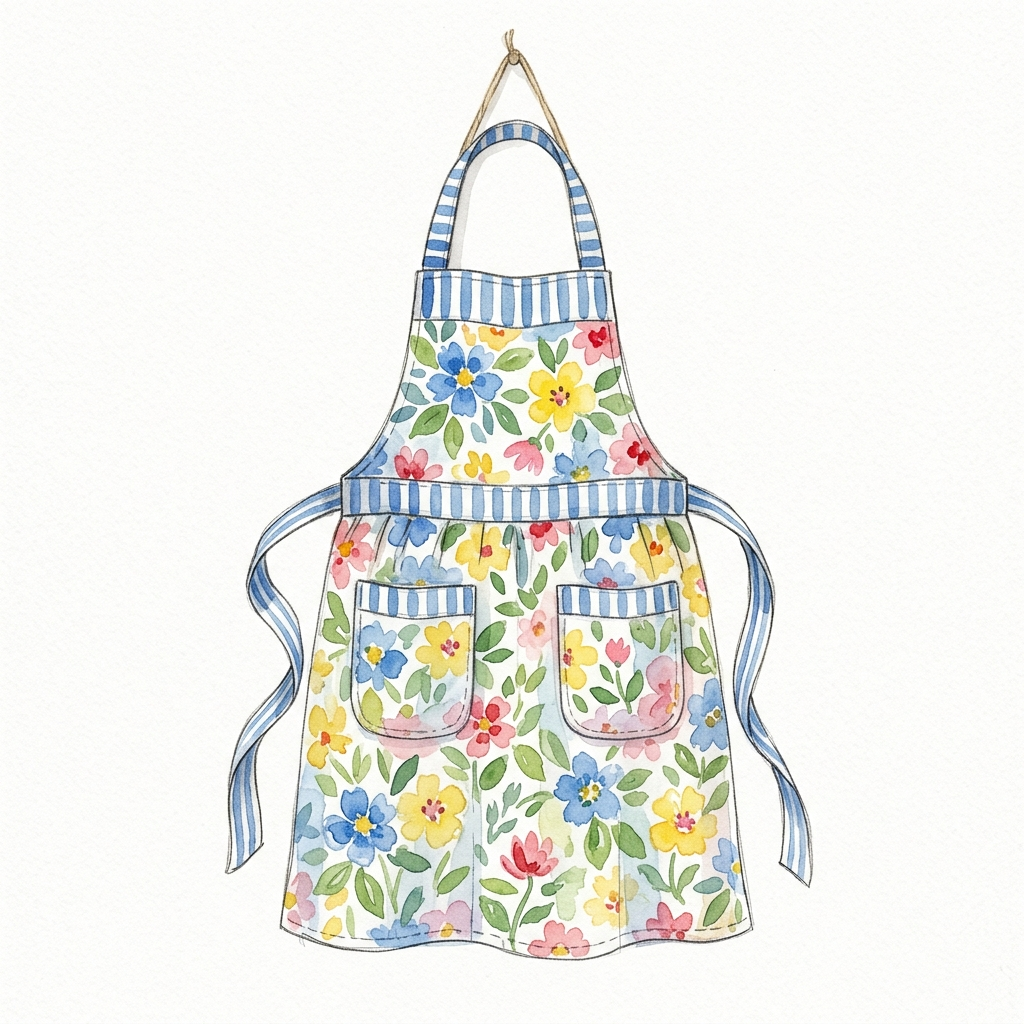
\includegraphics[width=0.85\linewidth,height=4cm,keepaspectratio]{vokab_300dpi/schiertech.png} \\
            \small\textit{De Schiertech (Tablier / Apron)}
            \vspace{0.3cm}
        }}
    \end{minipage}

    \vspace{1.5em}

    \begin{minipage}[t]{0.48\textwidth}
        \centering
        \textbf{E Schneidbriet}
        \vspace{0.5em}
        \framebox{\parbox{0.9\linewidth}{\centering
            \vspace{0.3cm}
            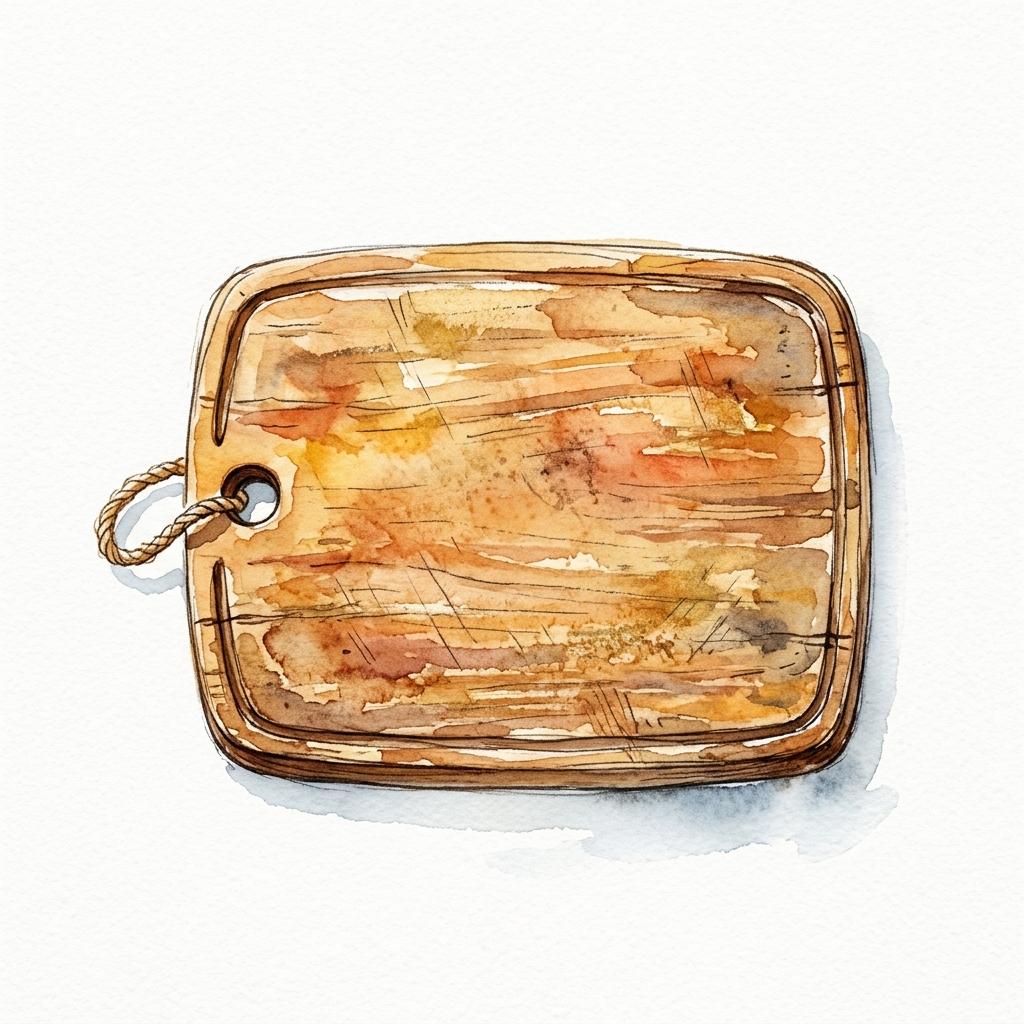
\includegraphics[width=0.85\linewidth,height=4cm,keepaspectratio]{vokab_300dpi/schneidbriet.png} \\
            \small\textit{Dat Schneidbriet (Planche à découper / Cutting board)}
            \vspace{0.3cm}
        }}
    \end{minipage}
    \hfill
    \begin{minipage}[t]{0.48\textwidth}
        \centering
        \textbf{E Rack}
        \vspace{0.5em}
        \framebox{\parbox{0.9\linewidth}{\centering
            \vspace{0.3cm}
            
\includegraphics[width=0.85\linewidth,height=4cm,keepaspectratio]{vokab_300dpi/rack.png} \\
            \small\textit{De Rack (Robe / Dress)}
            \vspace{0.3cm}
        }}
    \end{minipage}

    \vspace{1.5em}

    \begin{minipage}[t]{0.48\textwidth}
        \centering
        \textbf{D'Strëmp}
        \vspace{0.5em}
        \framebox{\parbox{0.9\linewidth}{\centering
            \vspace{0.3cm}
            
\includegraphics[width=0.85\linewidth,height=4cm,keepaspectratio]{vokab_300dpi/stremp.png} \\
            \small\textit{D'Strëmp (Chaussettes / Socks)}
            \vspace{0.3cm}
        }}
    \end{minipage}
    \hfill
    \begin{minipage}[t]{0.48\textwidth}
        \centering
        \textbf{E Puppelchen}
        \vspace{0.5em}
        \framebox{\parbox{0.9\linewidth}{\centering
            \vspace{0.3cm}
            
\includegraphics[width=0.85\linewidth,height=4cm,keepaspectratio]{vokab_300dpi/puppelchen.png} \\
            \small\textit{De Puppelchen (Bébé, poupée / Baby, doll)}
            \vspace{0.3cm}
        }}
    \end{minipage}

    \vspace{1.5em}

    \begin{minipage}[t]{0.48\textwidth}
        \centering
        \textbf{E Rank}
        \vspace{0.5em}
        \framebox{\parbox{0.9\linewidth}{\centering
            \vspace{0.3cm}
            
\includegraphics[width=0.85\linewidth,height=4cm,keepaspectratio]{vokab_300dpi/rank.png} \\
            \small\textit{De Rank (Anneau, bague / Ring)}
            \vspace{0.3cm}
        }}
    \end{minipage}
    \hfill
    \begin{minipage}[t]{0.48\textwidth}
        \centering
        \textbf{E Brout}
        \vspace{0.5em}
        \framebox{\parbox{0.9\linewidth}{\centering
            \vspace{0.3cm}
            
\includegraphics[width=0.85\linewidth,height=4cm,keepaspectratio]{vokab_300dpi/brout.png} \\
            \small\textit{Dat Brout (Pain / Bread)}
            \vspace{0.3cm}
        }}
    \end{minipage}
\end{center}


